\chapter{Das Verfahren in der Theorie}
In diesem Kapitel wird auf die theoretischen Grundlagen des Verfahrens eingegangen. Es handelt sich dabei um eine Zusammenfassung, welche die wichtigsten Konzepte für das weitere Verständnis aufbereiten soll und beschränkt sich daher auf das Wesentliche. Weiterführende Lektüre, welche für die folgenden Abschnitte auch als Quelle gedient hat, ist unter anderem zu finden bei \cite{Simek:12}, \cite{Mathworks:17b} oder \cite{Rahmann}.

\section{Das mathematische Modell einer Kamera}
Das Lichtschnittverfahren macht sich nicht nur den eingangs erwähnten Laser zu Nutze, sondern nutzt zusätzlich eine Kamera um die räumlichen Informationen des vermessenen Objektes zu rekonstruieren. Die Kamera dient dabei als Betrachter der projizierten Laserlinie. Mathematisch wird hier das Modell einer Lochkamera zugrunde gelegt. Bei diesem Modell wird angenommen, dass Lichtstrahlen, die von einem Objekt reflektiert werden, durch den Fokuspunkt der Kamera fallen, dort gebündelt werden, und anschließend auf der anderen Seite des Fokuspunktes auf eine gegenüberliegende Projektionsfläche geworfen werden. So entsteht auf der Projektionsfläche das invertierte Bild des Objektes. Abb. \ref{fig:lochkamera} verdeutlicht das Modell. 

\begin{figure}
\centering \includegraphics{images/lochkamera.png}
\caption[Modell einer Lochkamera]{Modell einer Lochkamera. Quelle: \cite{Mathworks:17b}}\label{fig:lochkamera}
\end{figure}

Es handelt sich also um eine Projektion vom dreidimensionalen Raum, dem Weltkoordinatensystem, auf eine zweidimensionale Fläche, im Folgenden als Bildebene bezeichnet. Wie diese Projektion stattfindet, hängt vor allem von zwei Kamera-abhängigen Sets an Parametern ab: Den intrinsischen und den extrinsischen Kameraparametern. Erstere hängen lediglich von der Beschaffenheit der Kamera ab und ändern sich nicht wenn die Kamera ihre Position im Raum ändert. Hierunter fallen die Brennweite der Kamera ("`Focal length'' in der oben stehenden Abbildung) sowie der Ursprung des Bildebenenkoordinatensystms. Außerdem wird hierüber eine Scherung des projizierten Bildes bestimmt. Die intrinsischen Parameter können als 

\begin{equation}
K = \begin{pmatrix}
f_x & s & x_0 \\
0 & f_y & y_0 \\
0 & 0 & 1 
\end{pmatrix}
\end{equation}

 in einer Matrix zusammengefasst werden, in welcher \(f_x\) und \(f_y\) für die Brennweite in Pixeln (bei perfekt quadratischen Pixeln gilt \(f_x = f_y\)), \(s\) für die Scherung und \(y_0\) sowie \(x_0\) für die Verschiebung des Bildkoordinatenursprung in \(X\)- und \(Y\)-Richtung in Pixeln stehen. 
\newline
Im Gegensatz dazu definieren die extrinsischen Parameter die Orientierung und die Position der Kamera im Weltkoordinatensystem. Entsprechend werden diese als eine Rotationsmatrix \(R\) und ein Ortsvektor \(T\) ausgedrückt. Dabei handelt es sich bei \(T\) jedoch nicht etwa um die Position der Kamera in Weltkoordinaten, sondern um den Ursprung des Weltkoordinatensystems welcher in dem Koordinatensystem ausgedrückt ist, dessen Ursprung in der Kamera liegt.
\newline
Mithilfe dieser Parameter ergibt sich die Kameramatrix \(P\) als
\begin{equation}
	P = K \big[ R \mid T \big] 
\end{equation}
Sei nun 
\begin{equation}
	\vec{z_{W}} = \left(\begin{array}{c}x\\y\\z\\1\end{array}\right)
\end{equation}
ein Punkt im Weltkoordinatensystem, ausgedrückt in homogenen Koordinaten. Dann lässt sich der projizierte Bildpunkt
\begin{equation}
	\vec{z_{B}} = \left(\begin{array}{c}u\\v\\1\end{array}\right)
\end{equation}
wie folgt berechnen:
\begin{equation}
	\vec{z_{B}} = P * \vec{z_{W}}
\end{equation}

\newpage

\subsection{Die Kamerakalibrierung}
\label{subsec:KameraKalibrierungTheorie}

\subsubsection{Das Kalibrierungsmuster}
Um das Lichtschnittverfahren einzusetzen, müssen die internen und die externen Kameraparameter bekannt sein. Die Berechnung dieser Parameter geschieht in einem Prozess namens Kamerakalibrierung. Dabei wird mit der Kamera ein bestimmtes Muster fotografiert, welches es besonders einfach macht, algorithmisch Punkte in diesem Muster zu bestimmen. Ein üblicher Ansatz ist es, als ein solches Muster ein Schachbrettmuster mit einer bekannten Seitenlänge für die einzelnen Quadrate zu verwenden. So wurde auch in der vorliegenden Arbeit verfahren. Das Muster ist in Abb. \ref{fig:Calibration} zu sehen. Dieses Muster legt in einem bestimmten Punkt den Koordinatenursprung des Weltkoordinatensystems fest und spannt zugleich die X-Y-Ebene auf. Durch die bekannte Seitenlänge können dann die Weltkoordinaten von weiteren Punkten im Muster bestimmt werden. Wenn die Kamera nun ein Bild des Musters gemacht hat, kann aus diesen Punkten eine Menge von Bildpunkten bestimmt werden, deren entsprechende Weltkoordinaten bekannt sind, und die alle auf der X-Y-Ebene liegen.

\begin{figure}
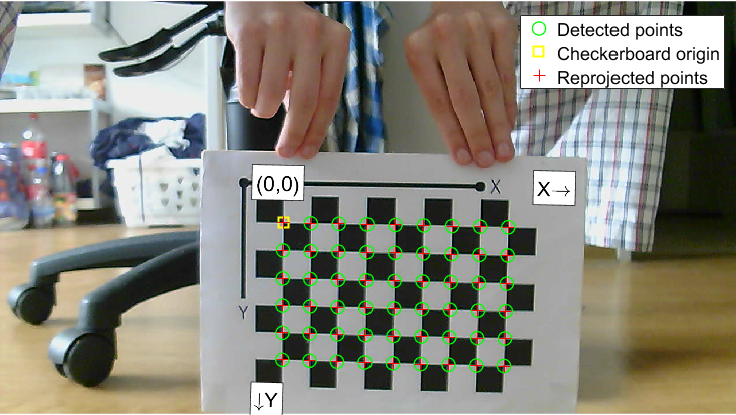
\includegraphics[width=\textwidth]{images/Calibration.png}
\caption{Ein Bild das für die Kalibrierung in Matlab benutzt wurde. Zu sehen ist das Schachbrettmuster mit einer Seitenlänge von 22 Millimetern für ein einzelnes Quadrat. Auf der Basis dieses Musters wird ein Set an Punkten im Weltkoordinatensystem generiert (dargstellt durch die grünen Kreise). Die roten Kreuze markieren die Projektionen dieser Punkte zurück auf die Bildebene nach der Kalibrierung. Der Ursprung des Weltkoordinatensystems befindet sich in der oberen linken Ecke des Schachbrettmusters (markiert durch ein gelbes Quadrat). Das Kalibrierungsmuster spannt so auch die X-Y-Ebene des Weltkoordinatensystems auf. }\label{fig:Calibration}
\end{figure}
 
\newpage

\subsubsection{Berechnung einer Homographie}
Alle Punkte, die im Kalibrierungsmuster erkannt wurden, befinden sich wie oben beschrieben auf der X-Y-Ebene. Für sie lässt sich also die Z-Koordinate auf null setzen. Die Projektion dieser Punkte vom Weltkoordinatensystem in die Bildebene kann also anstatt von einer Projektion vom 3D- in den 2D-Raum (wie bei anderen Punkten im Weltkoordinatensystem der Fall) als Projektion von einem 2D- in einen anderen 2D-Raum betrachtet werden. Eine solche Projektion kann als invertierbare projektive Transformation in Form einer Transformationsmatrix ausgedrückt werden. Transformationen dieser Art werden auch als Homographie bezeichnet und meistens mit \(H\) notiert. Aus einer einzelnen Fotografie des Kalibrierungsmusters kann eine solche Homographie \(H\) berechnet werden, indem die daraus resultierenden Korrespondenzen zwischen Punkten im Weltkoordinatensystem und ihren Projektionen auf der Bildeben betrachtet werden. Die Berechnung, welche angepasst aus \cite{Kriegman:07} übernommen wurde, läuft wie folgt ab:
\newline
Seien \(\vec{x_w} = \left(x_w y_w z_w\right)^{T}\) ein Punkt auf der Kalibrierungsmusterebene und \(\vec{x_b} = \left(x_b y_b z_b\right)^{T}\) ein Punkt auf der Bildebene, beide in homogenen Koordinaten. Dann gilt für die Homographie \(H\), dargestellt als \(3\times 3\)-Matrix:
\begin{equation}
\label{equ:homographie1}
	\left(\begin{array}{c}x_b\\y_b\\z_b\end{array}\right) =  \begin{pmatrix}
			H_{11} & H_{12} & H_{13} \\
			H_{21} & H_{22} & H_{23} \\
			H_{31} & H_{32} & H_{33}
		\end{pmatrix} * \left(\begin{array}{c}x_w\\y_w\\z_w\end{array}\right)
\end{equation}
Um homogene Koordinaten in ihr inhomogene Entsprechung umzuwandeln, werden sie durch die Koordinate der hinzugefügten Dimension geteilt. Es gilt für die entsprechenden inhomogenen Koordinaten \(x_b\prime\) und \(y_b\prime\) also:
\begin{equation}
\label{equ:homographie2}
	x_b\prime = \frac{x_b}{z_b} \;\;,\;\; x_b\prime = \frac{y_b}{z_b}
\end{equation} 
Sei nun o.B.d.A. \(z_w = 1\). Aus den Gleichungen \ref{equ:homographie1} und \ref{equ:homographie2} folgt dann:
\begin{gather}
\label{equ:homographie3}
	x_b\prime = \frac{H_{11}x_w + H_{12}y_w + H_{13}}{H_{31}x_w + H_{32}y_w + H_{33}} \Leftrightarrow \\
	x_b\prime \left( H_{11}x_w + H_{12}y_w + H_{13} \right) = H_{31}x_w + H_{32}y_w + H_{33}\Leftrightarrow \\
	x_b\prime \left( H_{11}x_w + H_{12}y_w + H_{13} \right) - \left( H_{31}x_w + H_{32}y_w + H_{33}\right) = 0
\end{gather}

\begin{gather}
\label{equ:homographie4}
	y_b\prime = \frac{H_{21}x_w + H_{22}y_w + H_{23}}{H_{31}x_w + H_{32}y_w + H_{33}} \Leftrightarrow \\
	y_b\prime \left( H_{21}x_w + H_{22}y_w + H_{23} \right) = H_{31}x_w + H_{32}y_w + H_{33}\Leftrightarrow \\
	y_b\prime \left( H_{21}x_w + H_{22}y_w + H_{23} \right) - \left( H_{31}x_w + H_{32}y_w + H_{33} \right) = 0
\end{gather}

Seien nun die Vektoren \(\vec{h}\), \(\vec{a_x}\), \(\vec{a_y}\) definiert als:
\begin{gather}
	\vec{h} = \left( H_{11}, H_{12}, H_{13}, H_{21}, H_{22}, H_{23}, H_{31}, H_{32}, H_{33} \right)^{T} \\
	\vec{a_x} = \left( -x_w, -y_w, -1, 0, 0, 0, x_b\prime x_w, x_b\prime y_w, x_b\prime \right)^{T} \\
	\vec{a_y} = \left( 0, 0, 0, -x_w, -y_w, -1, y_b\prime x_w, y_b\prime y_w, y_b\prime \right)^{T}
\end{gather}
Man kann \(\vec{a_{x}}\) und \(\vec{a_{y}}\) also aus einer Punktkorrespondenz von Weltkoordinaten zu Bildebenenkoordinaten bilden. Seien nun \(\vec{a_{xn}}\) und \(\vec{a_{yn}}\) die Vektoren die aus der \(n\)-ten Punktkorrespondenz gebildet wurden. Dann lässt sich eine Matrix \(A\) definieren mit:
\begin{equation}
	A = \left( \vec{a_{x1}}^{T}, \vec{a_{y1}}^{T}, \cdots , \vec{a_{xN}}^{T}, \vec{a_{yN}}^{T} \right)
\end{equation}
Nun sind alle Elemente  vorhanden um das lineare Gleichungssystem, mit dem wir \(H\) berechnen können, aufzustellen:
\begin{equation}
	A\vec{h} = 0
\end{equation}
Da die Homographie \(H\) mit jedem Skalierungsfaktor größer null multipliziert werden kann ohne dass sich die Transformation ändert, besitzt sie 8 Freiheitsgrade. Es reichen also mindestens 4 Punktkorrespondenzen aus damit das Gleichungssystem eindeutig für \(\vec{h}\) gelöst werden kann. 

\subsubsection{Bestimmung der Kameraparameter}
Aus jedem Bild des Kalibrierungsmusters kann also wie im vorangehenden Absatz beschrieben eine Homographie \(H\) berechnet werden. Nach \cite{Zhang:00} und \cite{Rahmann} können die Kameraparameter nun mittels dreier solcher Homographien wie folgt berechnet werden: 
\newline
Sei die Rotationsmatrix \(R = \left(\vec{r_1}\:\vec{r_2}\:\vec{r_3}\right)\) und die Translation \(T = \vec{t}\) der Kameramatrix dargestellt in ihren Spaltenvektoren. Für alle Punkte, aus denen eine bekannte Homographie \(H\) berechnet wurde, gilt, dass sie sich auf dem Kalibrierungsmuster (und damit auch auf der X-Y-Ebene) befinden. Daraus folgt, dass für jeden dieser Punkte \(\vec{x_{w}} = (X\:Y\:0\:1)^{T}\) und dessen Projektion auf die Bildebene \(\vec{x_{b}} = (U\:V\:1)^{T}\) gilt:
\begin{equation}
	\vec{x_{b}} = K\left(\:\vec{r_1}\:\vec{r_2}\:\vec{t}\:\right)\vec{x_{w}}
\end{equation}
Man beachte Ähnlichkeit zu Gleichung \ref{equ:homographie1}. Für die Homographie  \(H = \left(\vec{h_1}\:\vec{h_2}\:\vec{h_3}\right)\), dargestellt in ihren Spaltenvektoren, ergibt sich dann:
\begin{equation}
\label{equ:kameraparam3}
	\left(\:\vec{h_1}\:\vec{h_2}\:\vec{h_3}\:\right) = \lambda K\left(\:\vec{r_1}\:\vec{r_2}\:\vec{t}\:\right)
\end{equation}
mit \(\lambda\) als Skalar. Stellt man diese Gleichung geeignet um, ergibt sich für \(\vec{r_1}\) und \(\vec{r_2}\)
\begin{equation}
\vec{r_1} = \lambda^{-1} K^{-1}\vec{h_1} \;\;,\;\; \vec{r_2} = \lambda^{-1} K^{-1} \vec{h_2}
\end{equation}
Da für \(r_1\) und \(r_2\) gilt, dass sie orthogonal zueinander stehen (\(r_1^Tr_2=0\)) und normalisiert sind (\(\Vert r_1 \Vert = \Vert r_2 \Vert = 1\)), gilt:
\begin{equation}
\label{equ:kameraparam1}
	h_1^{T} K^{-T} K^{-1} h_2 = 0
\end{equation}
\begin{equation}
\label{equ:kameraparam2}
	h_1^{T} K^{-T} K^{-1} h_1 = h_2^{T} K^{-T} K^{-1} h_2
\end{equation}
Man erhält so zwei Bedingungen für die interne Kameramatrix \(K\). Möchte man alle fünf internen Kameraparameter bestimmen, sind also drei Homographien notwendig. Geht man davon aus, dass keine Scherung bei der Bildprojektion auftritt, kann auch mit zwei Homographien gearbeitet werden. Um die Bedingungen für \(K\) nun in die Form eines lösbaren linearen Gleichungssystems gießen zu können, sind einige weitere Definitionen von Nöten. Sei die Matrix \(B\) definiert als
\begin{equation}
	B = K^{-T}K^{-1} = \begin{pmatrix}
			B_{11} & B_{12} & B_{13} \\
			B_{21} & B_{22} & B_{23} \\
			B_{31} & B_{32} & B_{33}
		\end{pmatrix}
\end{equation}
mit einem zusammenfassenden Vektor
\begin{equation}
	\vec{b} = \left( B_{11}, B_{12}, B_{13}, B_{22}, B_{23}, B_{33} \right)^T
\end{equation}
Schreibt man nun den \(i\)-ten Spaltenvektor von \(H\) mit \(\vec{h_i} = \left( h_{i1}, h_{i2}, h_{j3} \right)^T\) lässt sich folgender Vektor 
\begin{equation}
	\vec{v_{ij}} = \left( h_{i1}h_{j1}, h_{i1}h_{j2}+h_{i2}h_{j1}, h_{i2}h_{j2},h_{i3}h_{j1}+h_{i1}h_{j3}, h_{i3}h_{j2}+h_{i2}h_{j3},h_{i3}h_{j3}\right)^T
\end{equation}
definieren. Die Bedingungen aus Gleichung \ref{equ:kameraparam1} und \ref{equ:kameraparam2} lassen sich dann in folgender Form aufstellen:
\begin{equation}
	\left( \begin{array}{c}\vec{v_{12}}^T\\\vec{v_{11}}^T - \vec{v_{22}}^T\end{array} \right)\vec{b} = 0
\end{equation}
Mit zwei anderen Homographien kann man dann eine \(6 \times 6\)-Matrix \(V\) durch Übereinanderstaplung von der entsprechenden \(\vec{v}\)-Vektoren, mit der sich dann folgendes eindeutig lösbare lineare Gleichungssystem ausdrücken lässt:
\begin{equation}
	V\vec{b} = 0
\end{equation}
Ist das Gleichungssystem gelöst und \(B\) durch \(\vec{b}\) bestimmt, kann man mittels einer Cholesky-Faktorisierung und einer Invertierung \(K\) bestimmen. Die externen Kameraparameter können für jede Aufnahme dann unter Anwendung der Gleichung \ref{equ:kameraparam3} für \(\lambda = \Vert K^{-1}\vec{h_1} \Vert\) folgendermaßen berechnet werden:
\begin{gather}
	\left(\vec{r_1},\vec{r_2},\vec{t}\right) = K^{-1}H \slash \Vert K^{-1}\vec{h_1} \Vert \\
	\vec{r_3} = \vec{r_1} \times \vec{r_2}
\end{gather}
Als Metrik zu Bestimmung der Güte der Kalibierung kann der sogenannte Reprojection Error berechnet werden, welcher auch von Matlab verwendet wird (vgl. \cite{Mathworks:17a} und \cite{StackOverflow:15}). Er ergibt sich aus den Pixelabständen zwischen den im Bild erkannten Schachbrett-Punkten und den auf das Bild mittels den Kameraparametern zurück projizierten korrespondierenden Weltkoordinaten, zu sehen auch in Abb. \ref{fig:Calibration}. Laut \cite{Mathworks:17a} gilt jeder durchschnittliche Fehler von unter einem Pixel als akzeptabel:
\begin{quotation}
"`As a general rule, reprojection errors of less than one pixel are acceptable.''
\end{quotation}
Bei dem in Bild aus Abb. \ref{fig:Calibration} wurde ein beispielsweise ein Repojection Error von 0.2 Pixeln erreicht.\newline
Auch wenn alle in diesem Kapitel aufgeführten linearen Gleichungssysteme theoretisch rein linear gelöst werden können, ist dies in der Praxis keine durchführbare Lösung. Durch Rauschen während der Messung würden keine verwendbaren Ergebnisse berechnet werden. Vielmehr wird ein Algorithmus angewandt, in dem das Problem als Minimierungsproblem formuliert und mittels der Minimum-Likelihood-Methode gelöst wird. Die Details dieses Ansatzes liegen jedoch außerhalb des Zuständigkeitsbereichs dieses Kapitels und können unter anderem bei \cite{Zhang:00} nachgelesen werden. Dort kann auch eingesehen werden wie mit Linsenverzerrung umgegangen wird, welche im hier beschriebenen Lösungsverfahren der Einfachheit halber ausgelassen wurde.

\section{Der Lichschnitt}
Die Kameramatrix \(P\) projiziert von einem dreidimensionalen Raum auf eine 2D-Bildebene. Dabei gehen die Tiefeninformationen verloren: Die Inverse dieser Matrix \(P^{-1}\) kann nicht eindeutig von einem 2D-Bildpunkt auf eine 3D-Weltkoordinate abbilden. Stattdessen bildet sie auf eine Gerade ab, die durch das Zentrum der Kamera und den von \(P\) projizierten Bildpunkt verläuft (siehe Abbildung \ref{fig:scanSchnitt}). Um nun zu rekonstruieren, wo auf dieser Geraden ein aufgenommener Punkt liegt und die vollständigen 3D-Koordinaten zu rekonstruieren, wird das Lichtschnittverfahren eingesetzt. Dabei wird von einem Laserlinienscanner eine Ebene aufgespannt, deren Parameter im Weltkoordinatensystem bekannt sind. Auf der Aufnahme eines zu vermessenen Objektes, welches sich mit der Ebene schneidet, ist dieser Schnitt in Form der auf das Objekt fallenden Laserlinie zu sehen. Jeder Punkt auf der Bildebene, der sich auf dieser Laserlinie befindet, liegt im Weltkoordinatensystem auch auf der aufgespannten Ebene. Es kann also der Schnittpunkt der Gerade, welche durch den Bildpunkt und das Kamerazentrum gegeben ist, und der durch den Laser definierten Ebene berechnet werden. Dieser Schnittpunkt ist dann in Weltkoordinaten gegeben. Wird dies mit allen auf der Laserlinie liegenden Bildpunkten gemacht, kann so eine Punktewolke der Schnittlinie der Ebene mit dem Objekt berechnet werden. Wie die Berechnung konkret stattfindet wird im Zuge von Abschnitt \ref{subsec:weltkoordinaten} beschrieben.\newline
Wurde das Objekt auch an anderen Stellen mit dem Laser abgetastet und abfotografiert, kann dieses Verfahren für jede Schnittlinie wiederholt werden. So kann eine Punktewolke berechnet werden, welche sich für jeden berechneten Schnittpunkt immer näher an das Objekt annähert. Wie das Verfahren für die vorliegende Ausarbeitung in die Praxis umgesetzt wurde, folgt im nächsten Kapitel.

\begin{figure}
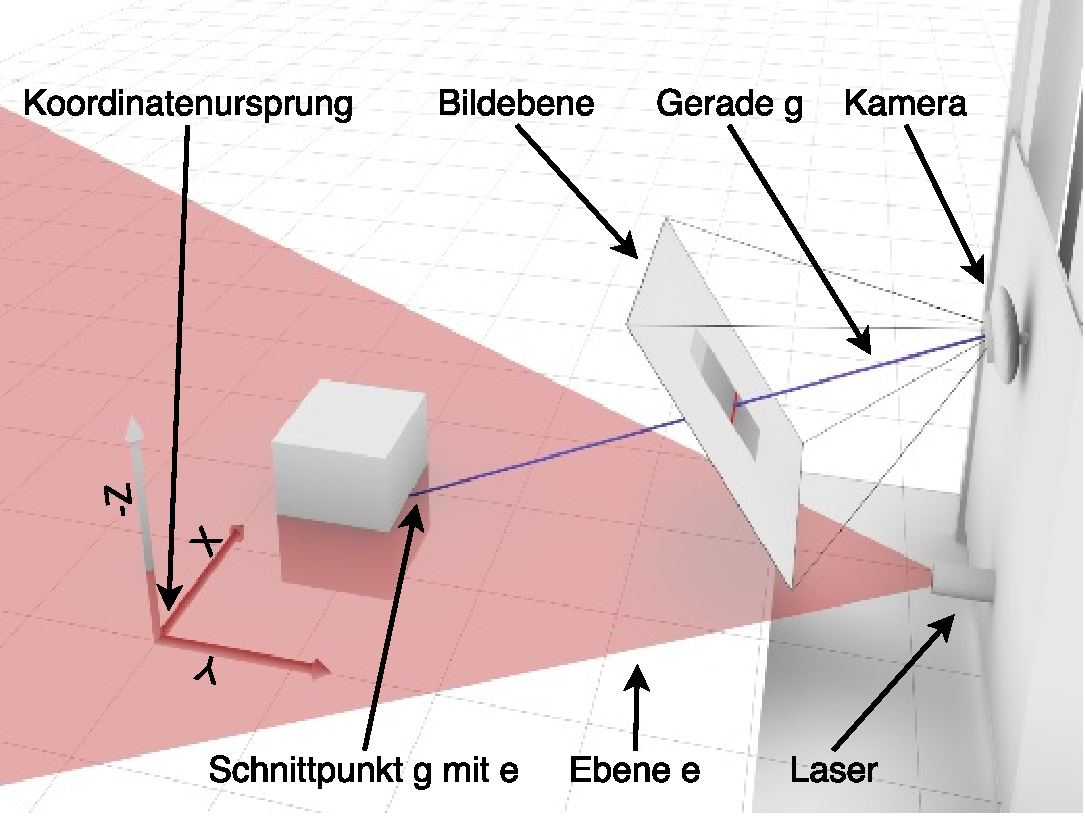
\includegraphics[width=\textwidth]{images/ScannerSchnitt.pdf}
\caption{Das Lichtschnittverfahren verbildlicht. Ein Punkt auf der Bildebene kann mit der inversen Kameramatrix auf eine Grade abgebildet werden, die durch den Punkt in der Bildebene und das Zentrum der Kamera verläuft. Die Tiefeninformationen werden berechnet in dem diese Gerade mit der vom Linienlaser aufgespannten Ebene geschnitten wird. Diese Operation wird für alle Punkte der Bildebene ausgeführt die auf der im Bild sichtbaren Laserlinie liegen.}\label{fig:scanSchnitt}
\end{figure}
